
\section{Simulation}\label{sec:simulation}


\subsection{1D mapping}

  \begin{figure}
\begin{center}
	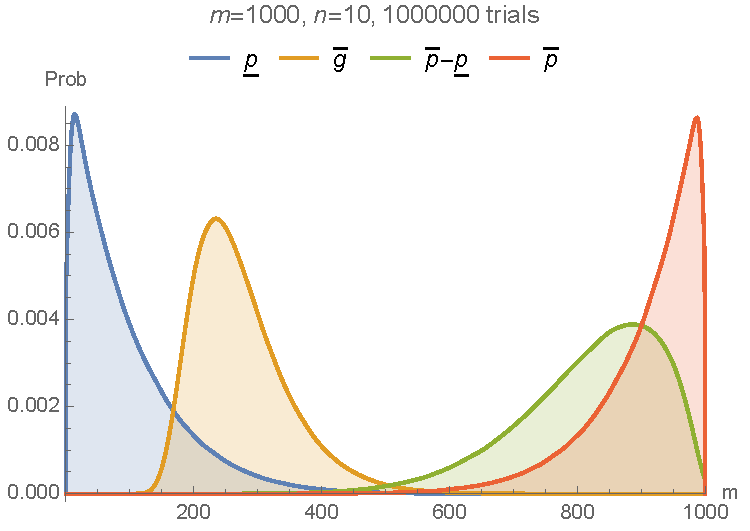
\includegraphics[width=1.0\columnwidth]{Prob1DcoverageGaps}
\end{center}
\caption{\label{fig:Prob1DcoverageGaps}
With a connected, 1D freespace $m$ = 1000 and $n=10$ particles, the distributions for the gap before the first $\overline{p}$ and after the last $\underline{p}$  gaps are symmetric. The maximum gap $\overline{g} \approx 250$.}
\end{figure}

\begin{figure}
\begin{center}
	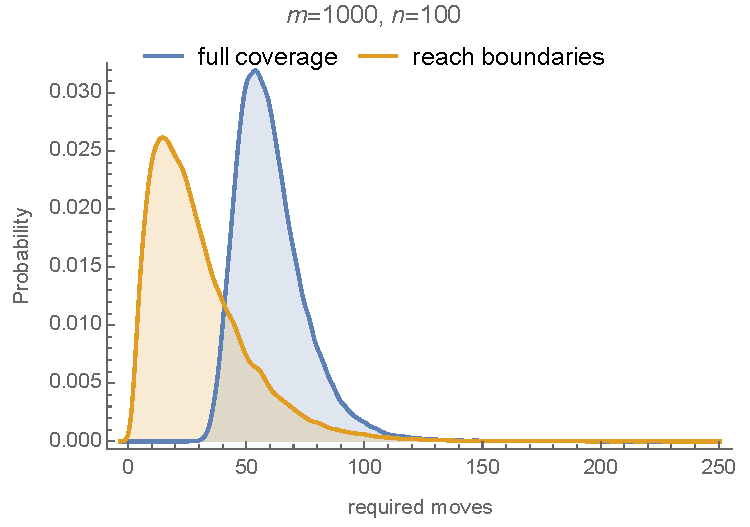
\includegraphics[width=1.0\columnwidth]{SimReachBoundaryCoverage}
\end{center}
\caption{\label{fig:SimReachBoundaryCoverage}
Full coverage in 1D requires 60.7 moves on average, while reaching the boundaries requires only 29.8.}
\end{figure}

  
 1D simulations were conducted in Mathematica, with code available at \cite{Arun2017GitHubUniformMapping}. 
 Fig.~\ref{fig:Prob1DcoverageGaps} shows the distributions for the minimum and maximum initial particle locations $\underline{p}$ and $\overline{p}$, the maximum gap $\overline{g}$, and the spread between the minimum and maximum $\overline{p}-\underline{p}$ for 1,000,000 Monte Carlo trials.
 The expected gap between the first particle and the boundary $\underline{p}$ is 90.94.
 The expected gap between the last particle and the boundary $\overline{p}$ is 90.98.
  The expected maximum gap is $\overline{g}$ is 273.9.
  
  Fig.~\ref{fig:SimReachBoundaryCoverage} shows that full coverage requires approximately twice the time required to explore the left and right boundaries when $m=1000$ and $n=100$.

  
  \subsection{2D mapping}  
  All simulations used maps with 5000 free cells.
  Each simulation trial was repeated 100 times.
  The number of particles ranged from 100 to 5000 by increments of 100.
  In each run except Fig.~\ref{fig:RegionvsFloodvsUniform} the particles were placed uniformly randomly throughout the workspace. 
  
 %%%%%%%%%%%%%%%  MappingAlg3maps
  The comparison plot Fig.~\ref{fig:MappingAlg3maps} between the mapping of  four 2D maps� \emph{H-tree}, \emph{complex}, \emph{empty rectangle} and \emph{linear} and a 1D map, shows that the H-tree map requires the most moves because it has the highest number of turns. 
  In Fig.~\ref{fig:MappingAlg3maps} there is an observable difference in moves between the linear and rectangular workspaces. 
	One reason is because the perimeter of the linear map is much larger than the rectangular map. 
	The number of cells to explore is $3m+2 = 15,002$ for the linear map, but only $m + 2(50+100) = 5,300$ for the rectangular map. 
	Only when the number of particles is around 2/3 of the number of free spaces is there an overlap between the moves taken to map the rectangular space and the linear space. 

 
\begin{figure}
\begin{center}
	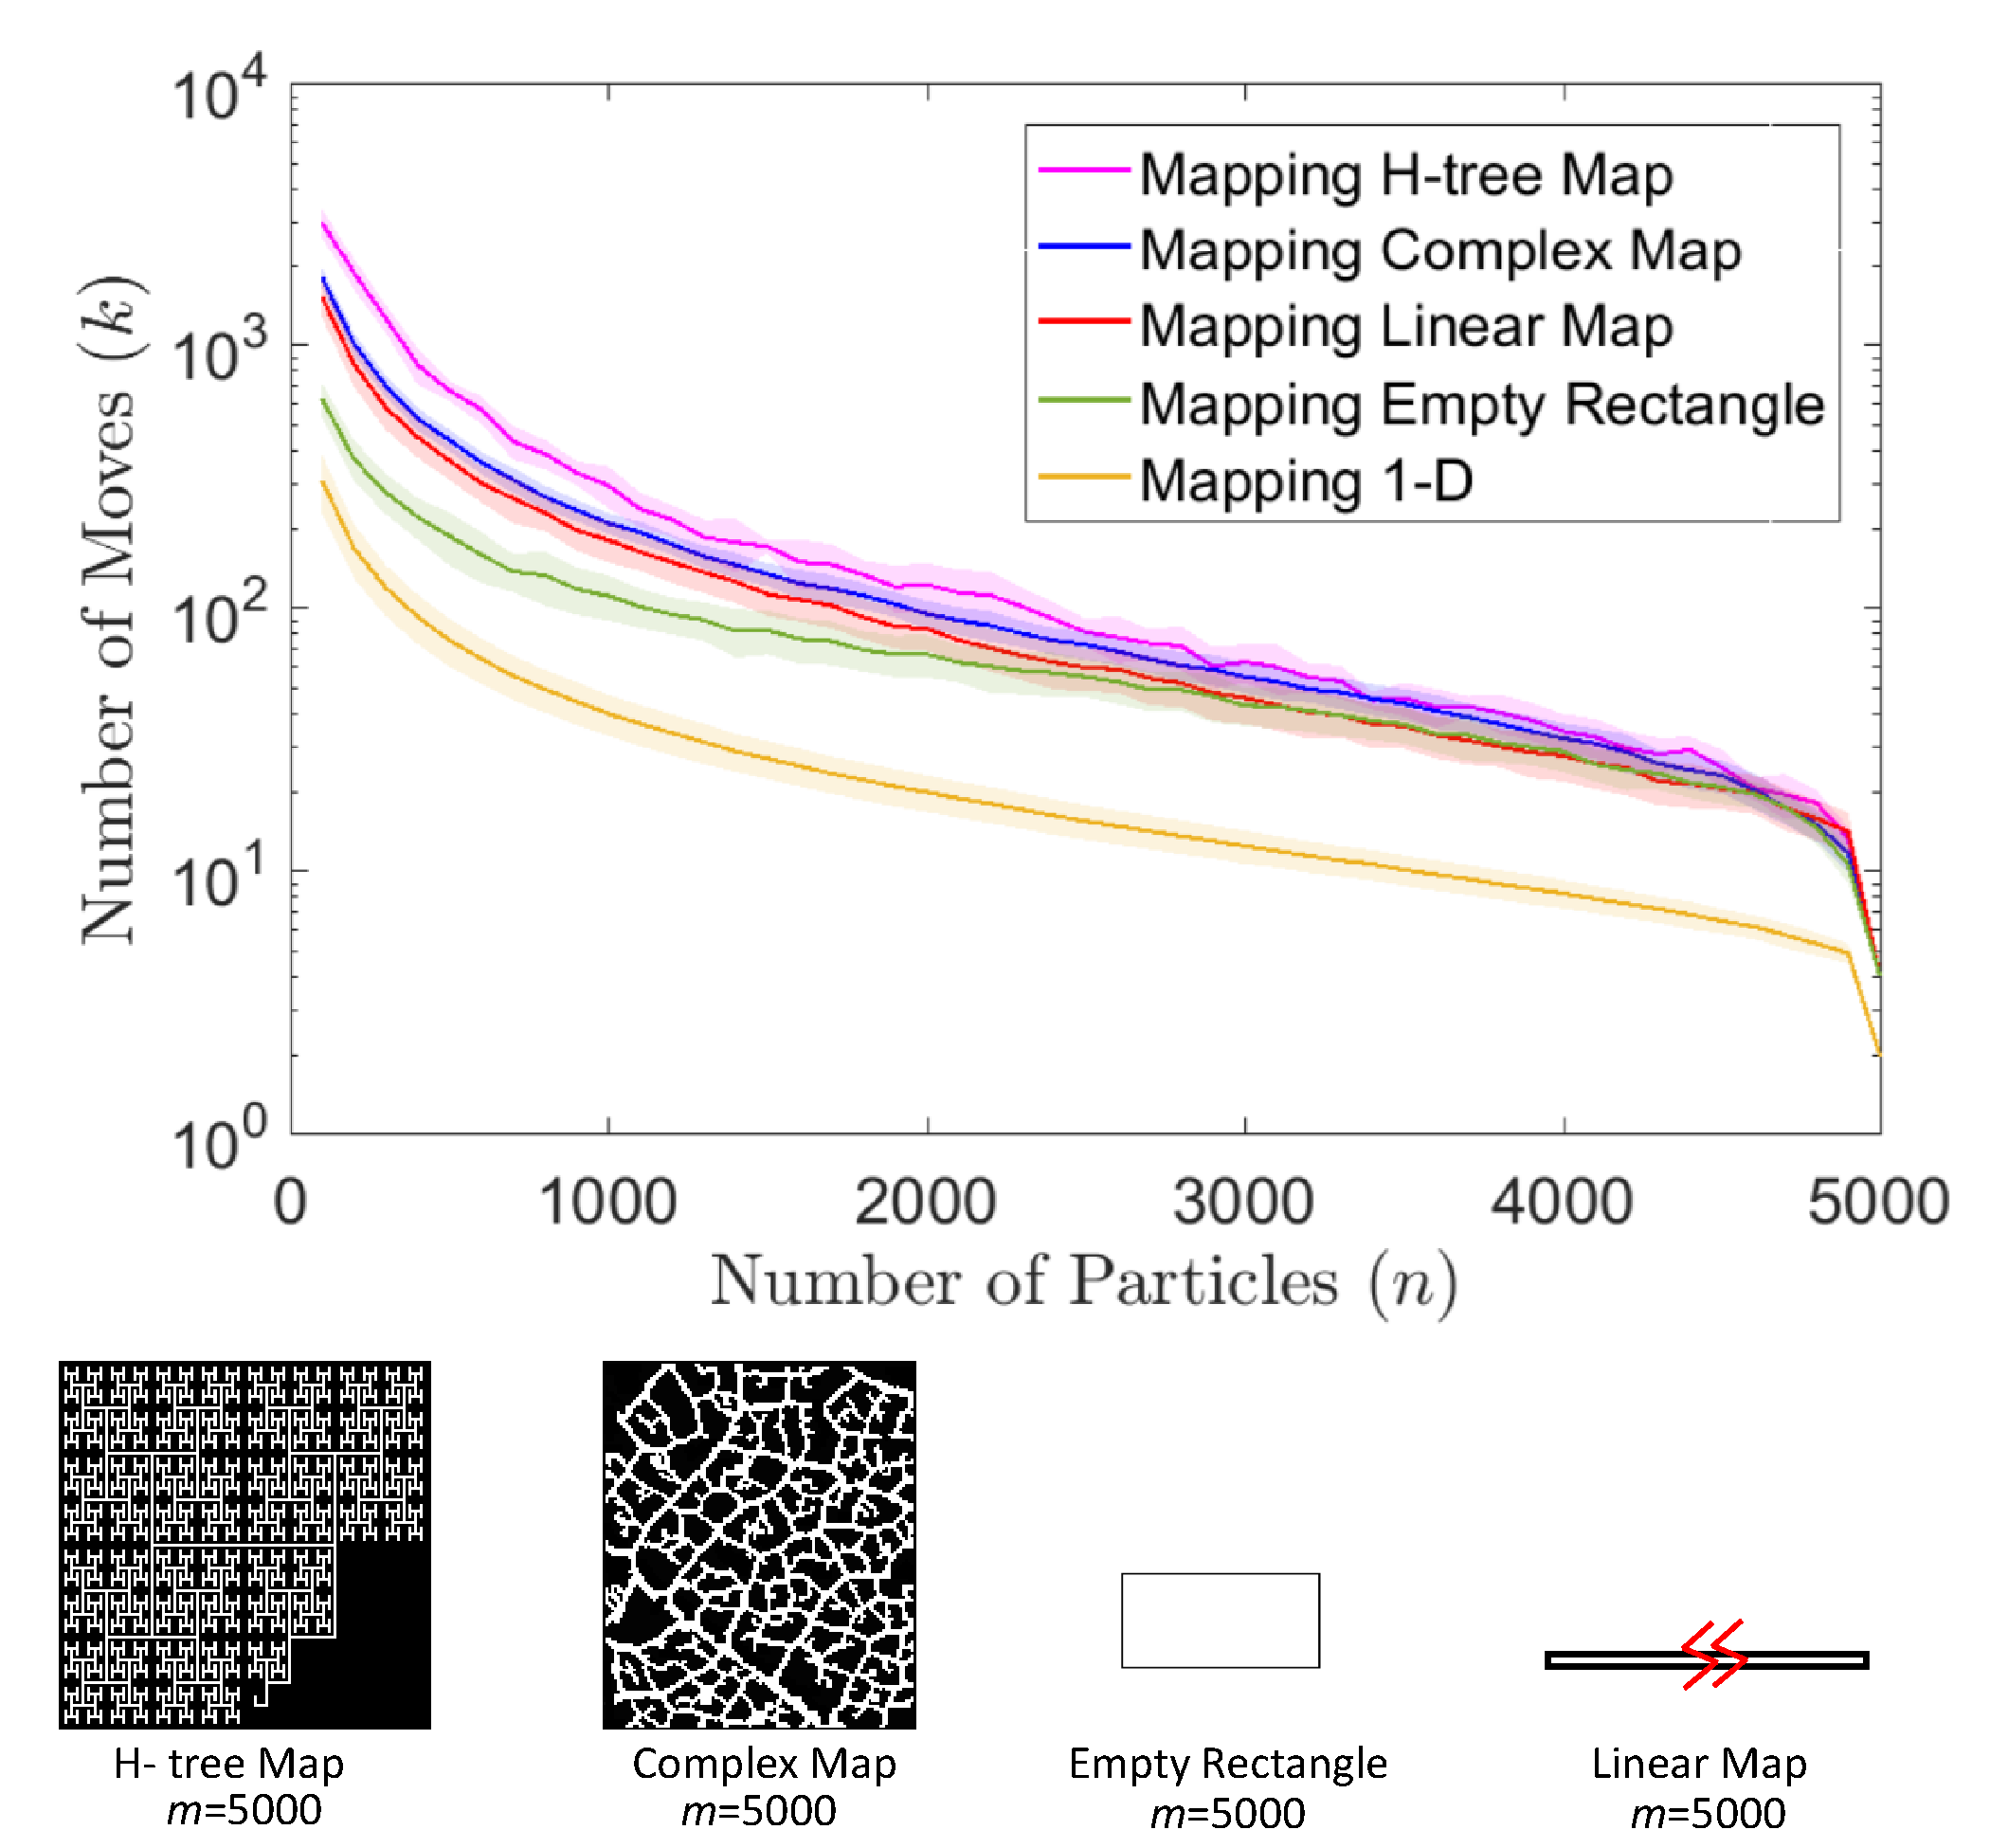
\includegraphics[width=1.0\columnwidth]{MappingAlg3maps}
\end{center}
\caption{\label{fig:MappingAlg3maps}
Comparison of mapping using the Closest Frontier algorithm on 2D maps of three types and 1D mapping on a linear map. 
Each map has 5000 free cells.
}
\end{figure}

 %%%%%%%%%%%%%%%  FrontierNodesVsk.pdf
The difference between algorithms is highlighted in Fig.~\ref{fig:FrontierNodesVsk}, which shows the number of frontier cells as a function of the number of moves commanded. All tests used $n=1000$ particles. Elect Particle requires on average twice as many moves as Closest Frontier and Random Moves requires ten times as many moves as closest Frontier.
The deviations for the Closest Frontier is also much lesser than the other two as seen from \ref{fig:FrontierNodesVsk} and Fig.~\ref{fig:Alg_linlogplot}.
	
\begin{figure}
\begin{center}
	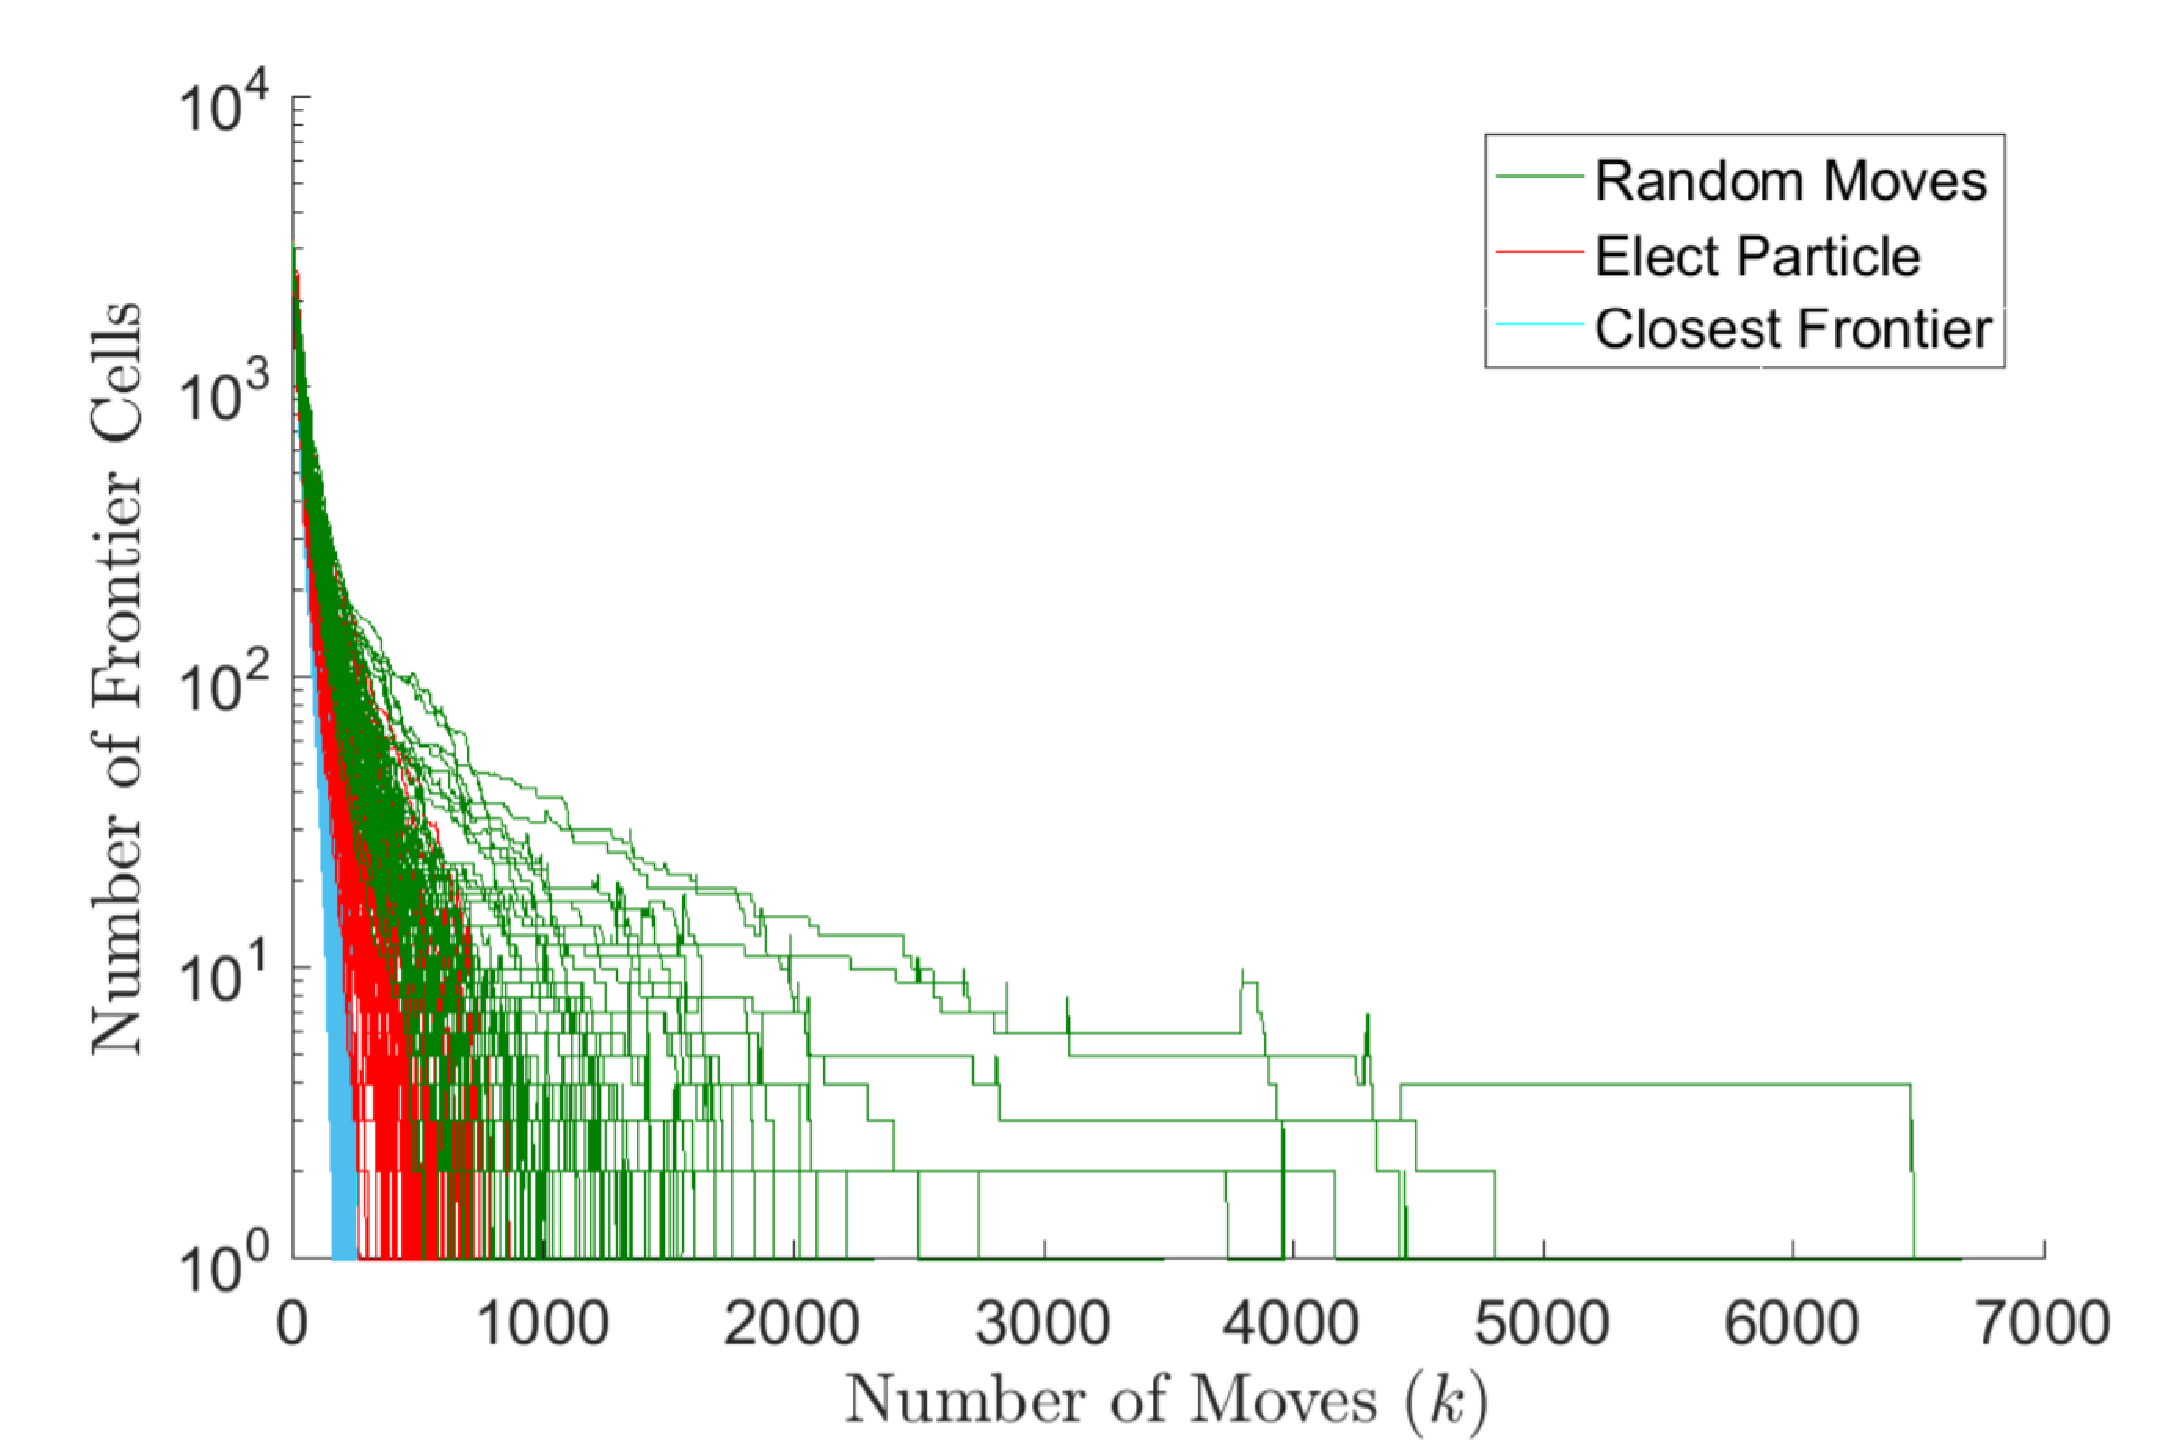
\includegraphics[width=1.0\columnwidth]{FrontierNodesVsklinlog.pdf}
\end{center}
\vspace{-2em}
\caption{\label{fig:FrontierNodesVsk}
Performing mapping on the complex 2D map with $n=1000$ particles. Random moves requires an average of 1683 moves. Elect particle requires 578 moves and Closest Frontier requires 215 moves}
\end{figure}	


%%%%%%%%%%%%%%%  fig:Alg_linlogplot

Fig.~\ref{fig:Alg_linlogplot} compares the performance of Algs.~\ref{alg:randommove}, \ref{alg:ElectParticle}, and \ref{alg:ClosestFrontier} on the complex 2D map. 
 For all algorithms  the mean completion time and standard deviation of the completion time decreased with increasing numbers of particles. 
Random moves performs worst, with the largest number of required moves and the largest standard deviation of required moves.  Random moves is slightly better than elect particle  for large numbers of particles, but both algorithms are beat by closest frontier, which has the minimum number of required moves and the smallest standard deviation.
  The maximum number of moves required using the closest frontier algorithm was for $k$=100 with an average of $\approx$1816 moves and standard deviation of 160 moves.
This reduces to four moves with 0 standard deviation when $n$= 5000 (the total number of free spaces).
%  The log plot shows that all three algorithms have an almost logarithmic relationship between $m$, the number of free spaces, and $k$, the number of particles.    % I don�t think we can claim this.  You'd have to fit a logrithmic fit to the data.  Try to do this with the linear-linear version of this data -- is it logarithmic?

\begin{figure}
\begin{center}
	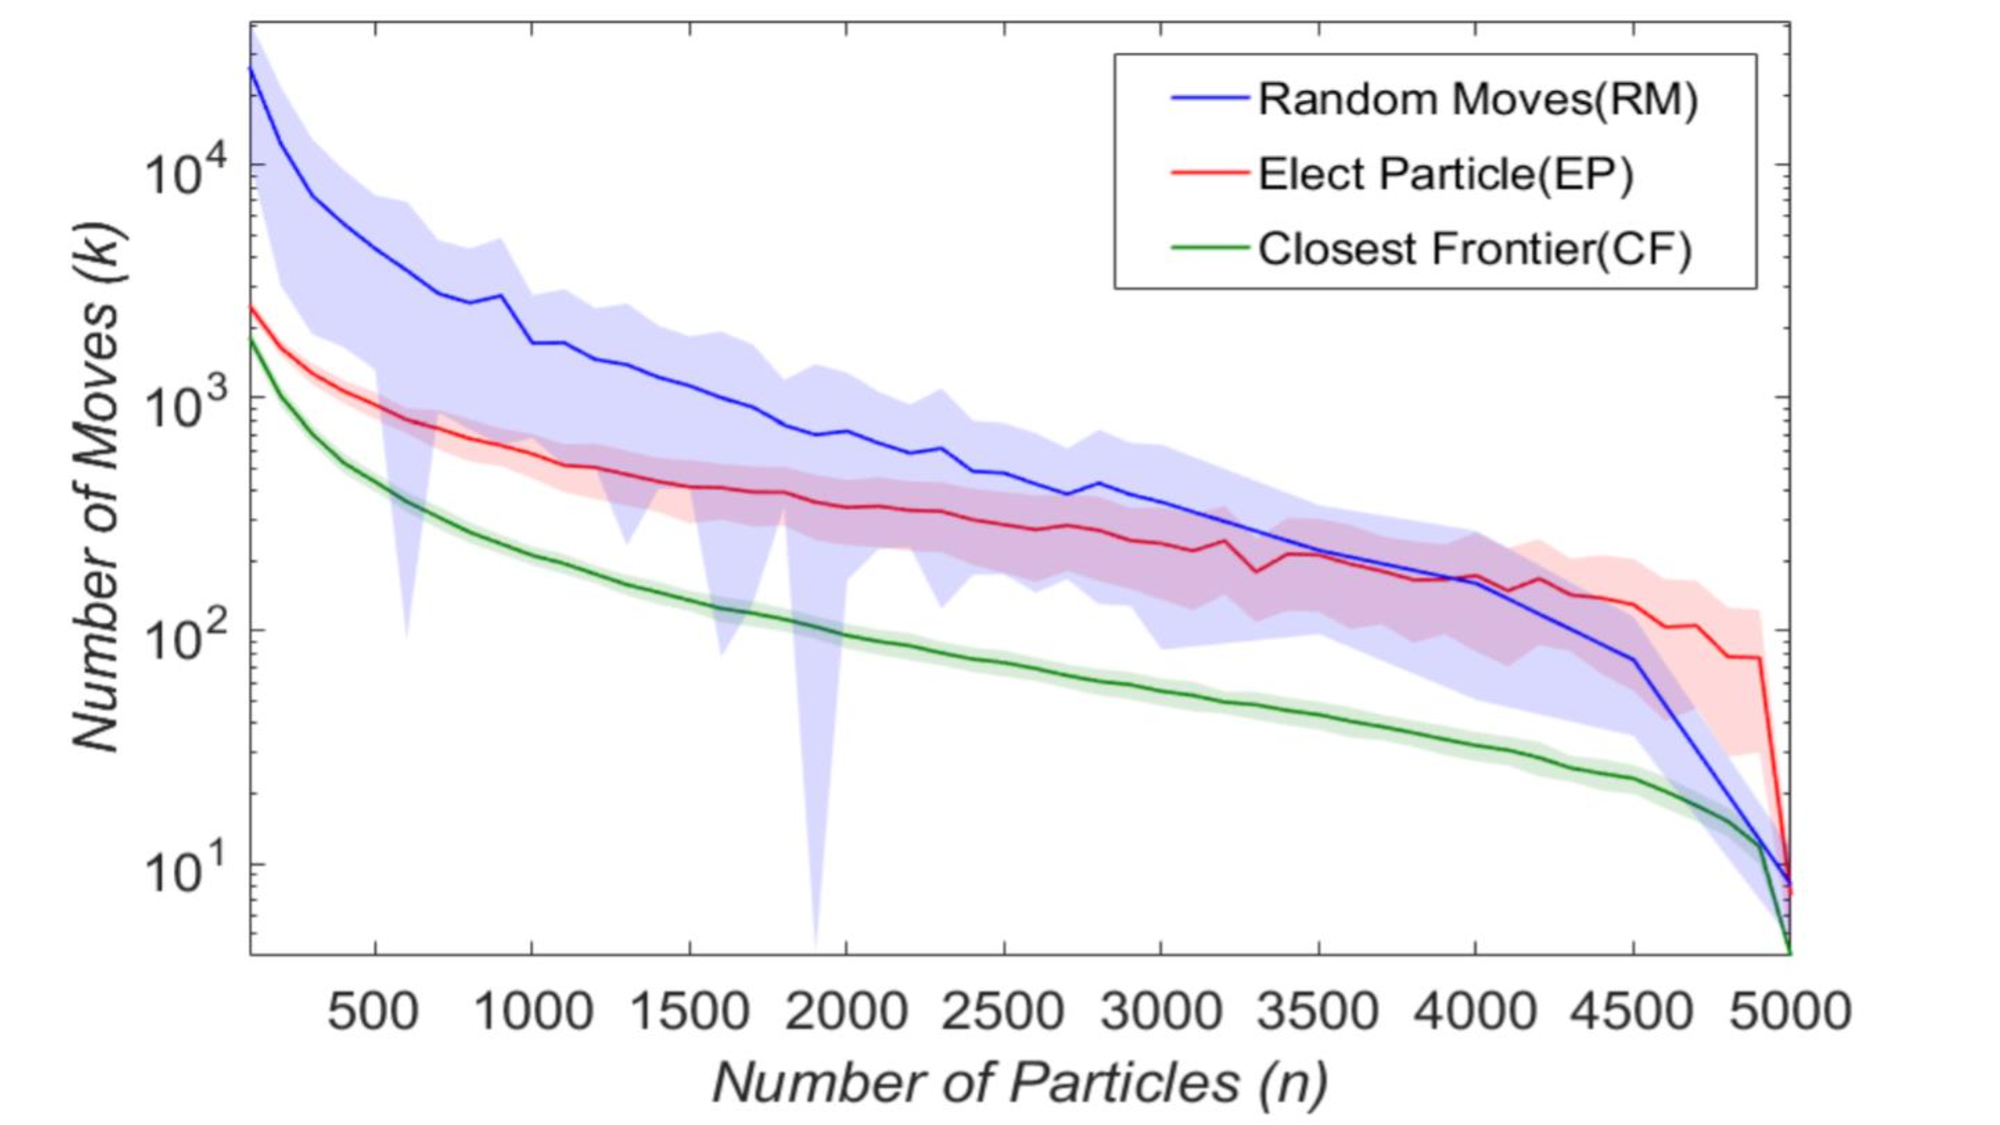
\includegraphics[width=1.0\columnwidth]{Alg_linlogplot}
\end{center}
\caption{\label{fig:Alg_linlogplot}
Comparison of three algorithms - Random Moves (blue), Elect Particle (red) and Closest Frontier (green) for mapping the 2D Complex Map of 5000 free spaces.}
\end{figure}

%%%%%%%%%%%%%%%  fig:CoverageMappingForaging
Fig.~\ref{fig:CoverageMappingForaging} compares mapping, coverage, and foraging on the complex 2D map.  All trials  used Alg.~\ref{alg:ClosestFrontier}. Coverage is performed with a known map, but with all free cells initialized to be frontier cells.  Similarly, foraging has a known map, but 10\% of the empty cells are labelled as frontier cells.  Foraging is easier than coverage and coverage is easier than mapping.

\begin{figure}
\begin{center}
	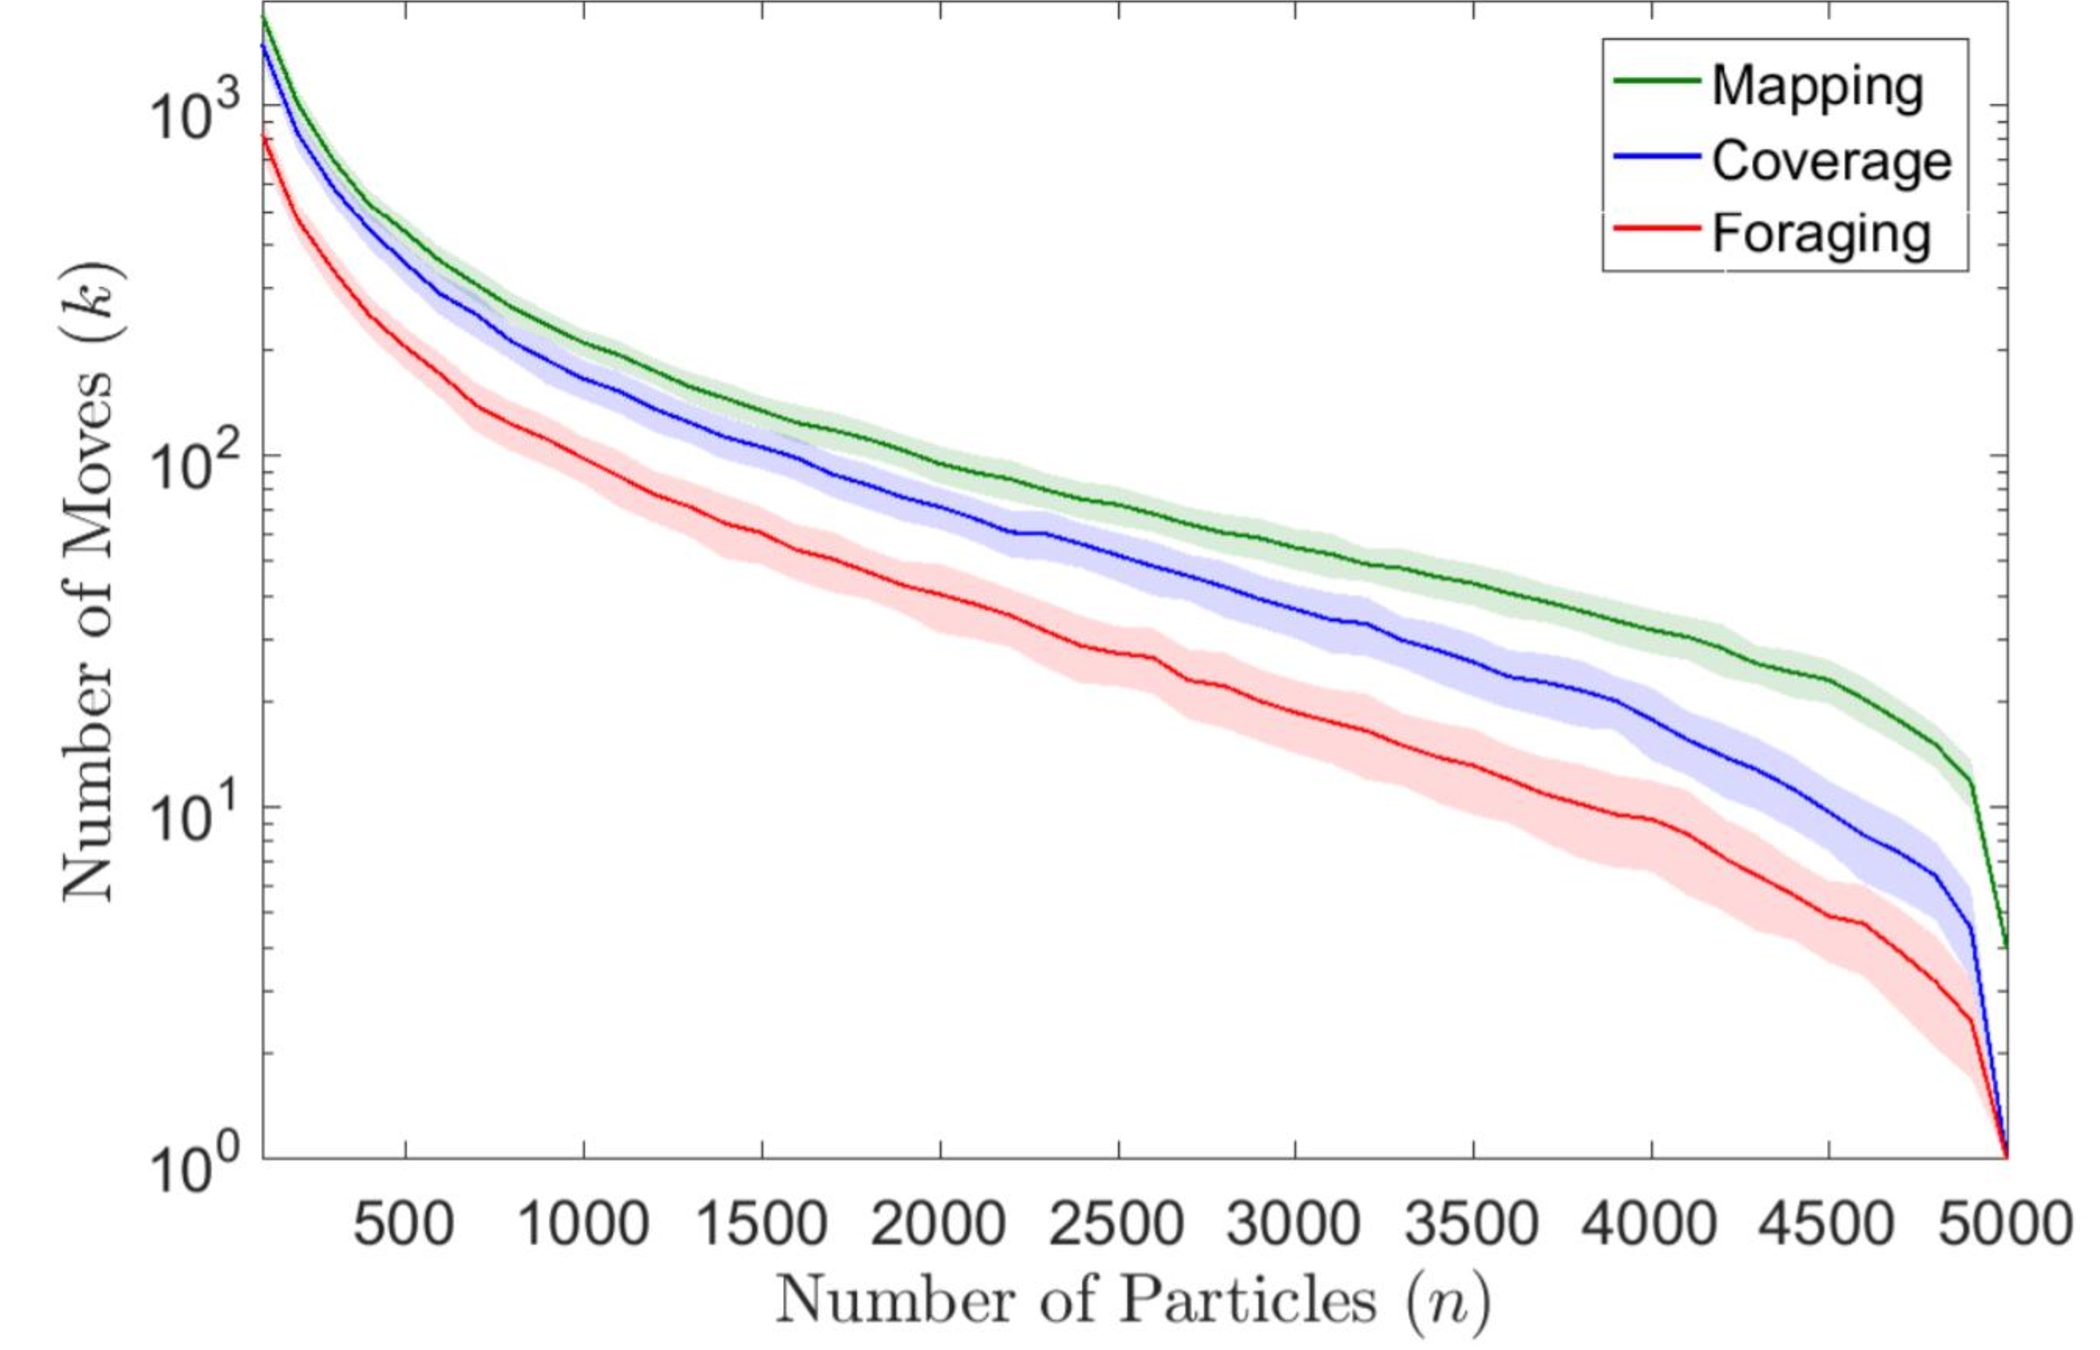
\includegraphics[width=1.0\columnwidth]{CoverageMappingForaging.pdf}
\end{center}
\caption{\label{fig:CoverageMappingForaging}
Comparison of three related problems:  mapping, coverage, and foraging on the complex 2D map.}
\end{figure}


%%%%%%%%%%%%%%%  fig:RegionvsFloodvsUniform
The final simulation test, shown in Fig.~\ref{fig:RegionvsFloodvsUniform}, compares the effect of different initial particle distributions in the complex 2D map.  
Region fill places all $n$ particles at a minimum Manhattan distance from a randomly selected location on the map.
Flood fill places one particle at a randomly selected location in the free space, and places the remaining particles according to a breadth-first expansion inside the free space.
Uniform distribution places the particles uniformly randomly.  
Region fill and flood fill have similar performance, while uniform distribution requires many fewer moves. 
This is because dispersing particles using only global inputs is difficult, and a uniform distribution starts with the particles dispersed, which allows it to map much faster.

\begin{figure}
\begin{center}
	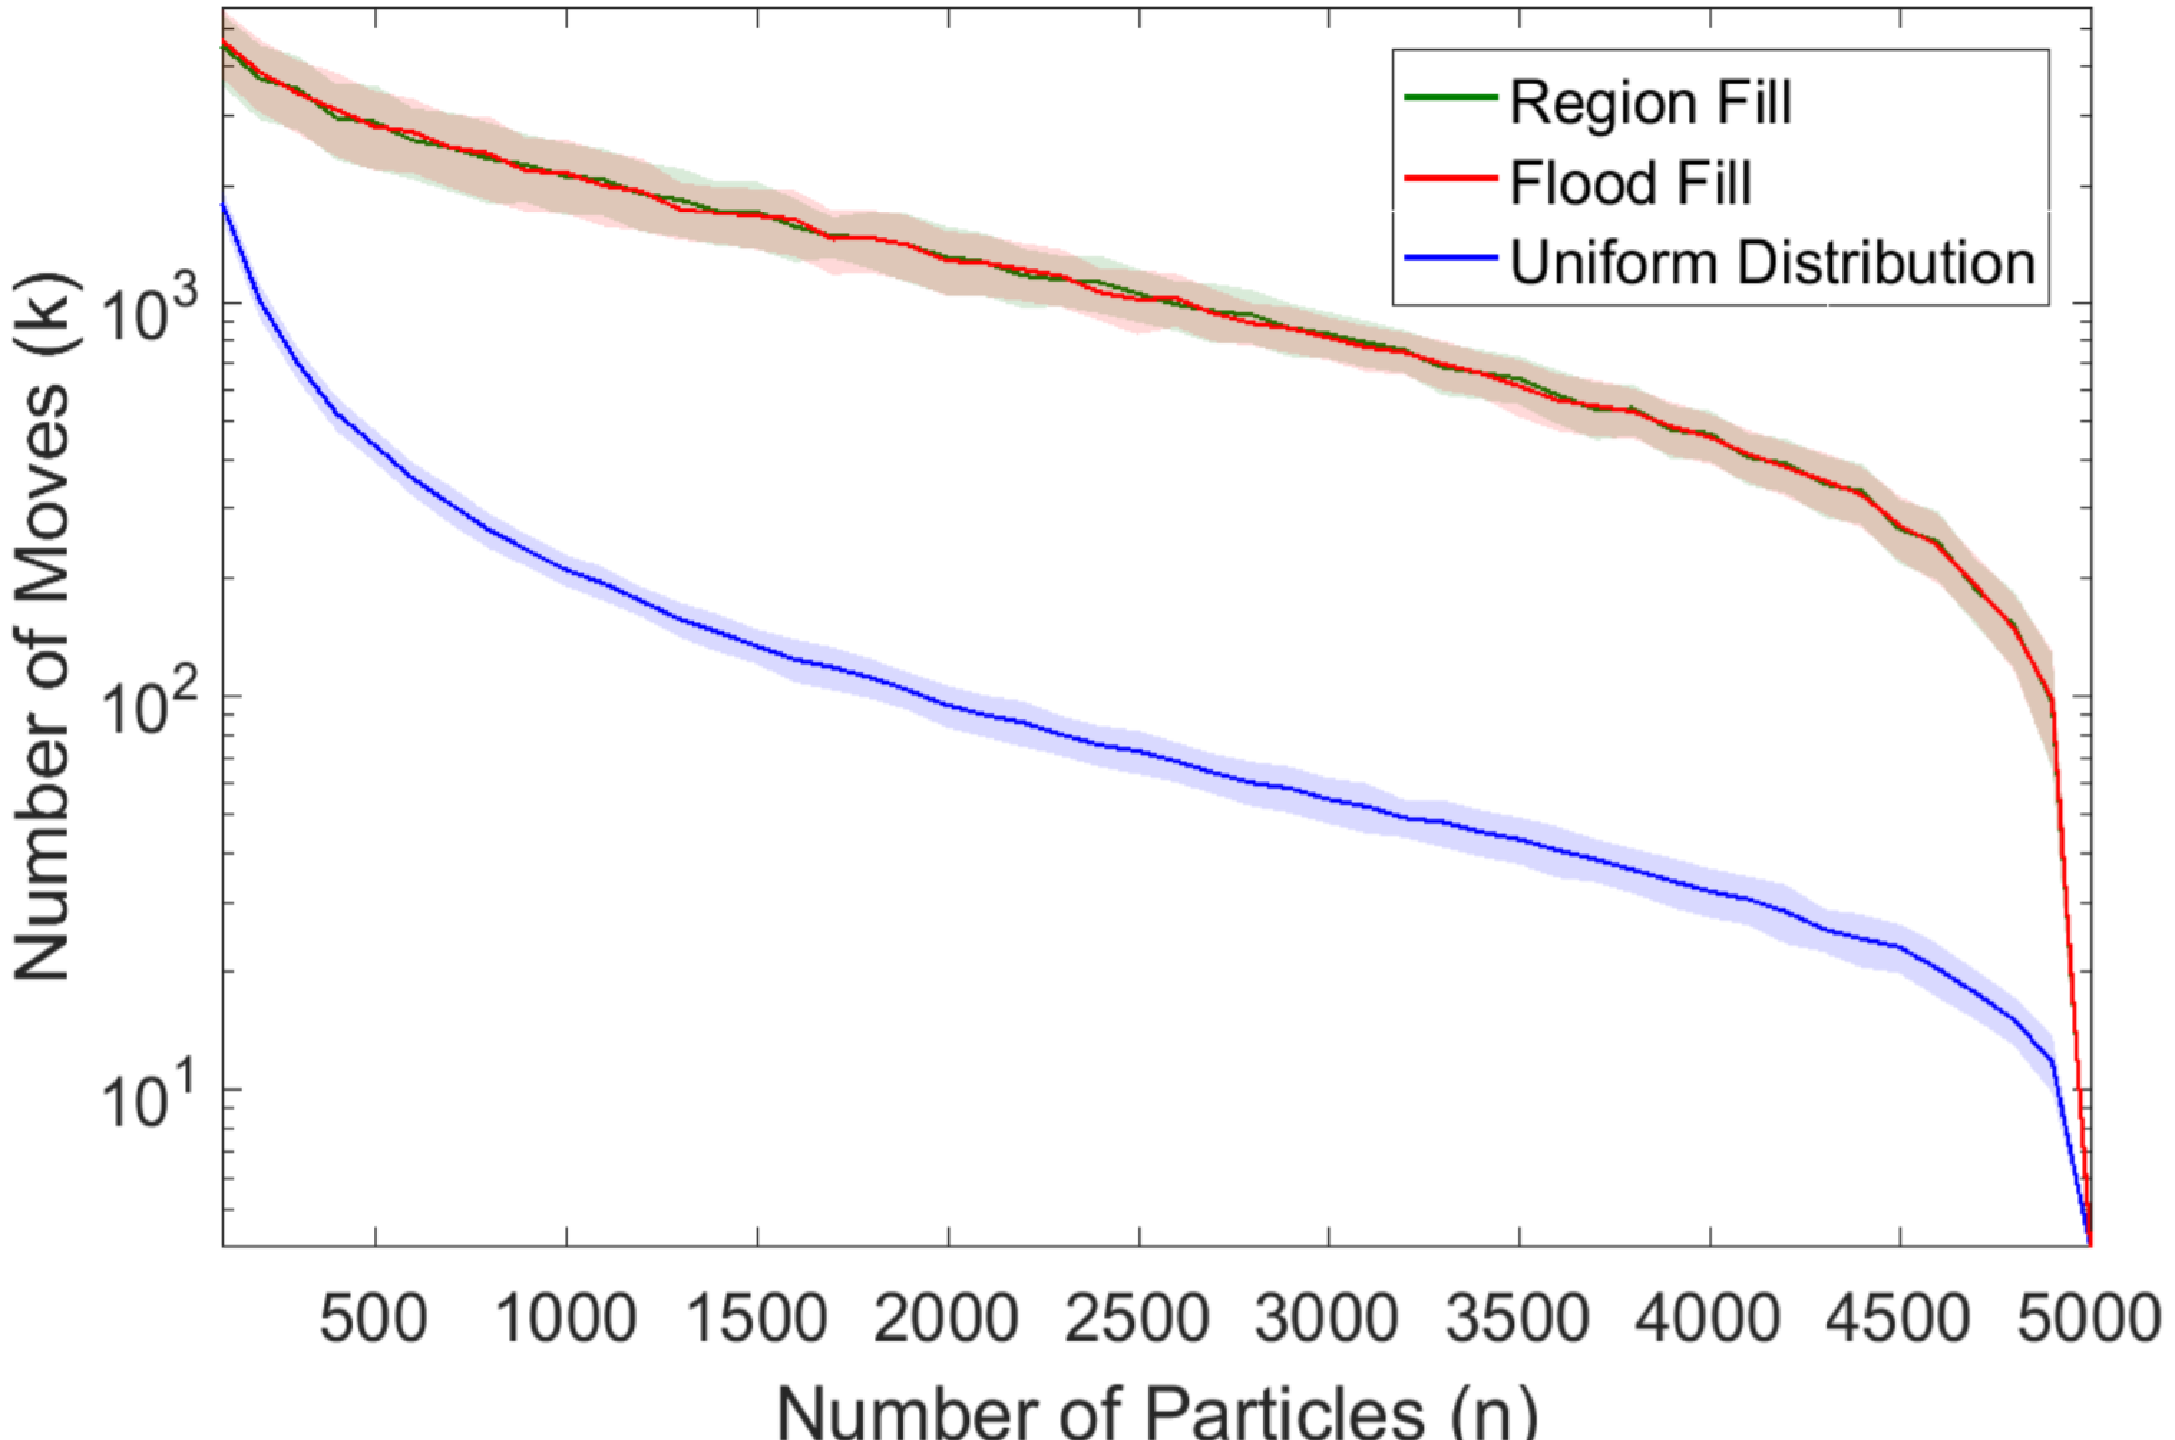
\includegraphics[width=1.0\columnwidth]{RegionvsFloodvsUniform.pdf}
\end{center}
\caption{\label{fig:RegionvsFloodvsUniform}
Comparison with different distributions:  flood-fill, region fill, and uniform distribution for mapping on the complex 2D map.  The results for flood-fill and region fill overlap. }
\end{figure}








